\subsection{Interprations of $Q_T(A,B)$}
Concider $n_a = |A| \times Q_T(A,B)$. 

\begin{definition}[Signature $S_{T,B}(A)$]
  Let $s_{T,B}(a) = |\{ b \in B : a \sim_T b \}|$.

  Let $(a_i)_{i \in [1 \ldots |A|]} \in A$ with $a_i \neq a_j$ for $i \neq j$.
  So $A = \{ a_i : i \in [1 \ldots |A|] \}$.

  Let $a_i$ is sorted in such way that $a_i \leq a_j$ for $i < j$.

  Define the signature $S_{T,B}(A)$ of $~_T$ for column $A$ to column $B$ as the following vector:
  \begin{equation}
    S_{T,B}(A) = (s_{T,B}(a_1), s_{T,B}(a_2), s_{T,B}(a_3), \ldots )
  \end{equation}
\end{definition}

The signature gives us a hint how the relation is distributed.
The sorting helps to normalize the signature and leads to lesser cases to consider as you could simply rename the items in the sets to get a equivalent relation with different sorting.

\begin{tabular}{c|c|l}
$Q_T(A,B)$ & $|A| \times Q_T(A,B)$ & signature $S_{T,B}(A)$ \\\hline
 0.000 & 0.000 & 1111 \\
 0.083 & 0.333 & 1112 \\
 0.167 & 0.667 & 1113 1122 \\
 0.250 & 1.000 & 1114 1123 1222 \\
 0.333 & 1.333 & 1124 1133 1223 2222 \\
 0.417 & 1.667 & 1134 1224 1233 2223 \\
 0.500 & 2.000 & 1144 1234 1333 2224 2233 \\
 0.583 & 2.333 & 1244 1334 2234 2333 \\
 0.667 & 2.667 & 1344 2244 2334 3333 \\
 0.750 & 3.000 & 1444 2344 3334 \\
 0.833 & 3.333 & 2444 3344 \\
 0.917 & 3.667 & 3444 \\
 1.000 & 4.000 & 4444
\end{tabular}
% \hfill
% \begin{tikzpicture}
% %Nodes
% \node  (nodeTitle) at (3,3.5) {Example for 1144};
% \node  (nodeA) at (0,3) {Alice};
% \node  (nodeB) at (0,2) {Bob};
% \node  (nodeC) at (0,1) {Charlie};
% \node  (nodeD) at (0,0) {Dave};
% \node  (nodeChocolate) at (6,3) {Chocolate};
% \node  (nodeVanilla)   at (6,2) {Vanilla};
% \node  (nodeBlueberry) at (6,1) {Blueberry};
% \node  (nodeRaspberry) at (6,0) {Raspberry};
% 
% %Lines
% \draw[->] (nodeA) edge node[thick, auto] {} (nodeChocolate);
% 
% \draw[->] (nodeB) edge node[thick, auto] {} (nodeVanilla);
% 
% \draw[->] (nodeC) edge node[thick, auto] {} (nodeRaspberry);
% \draw[->] (nodeC) edge node[thick, auto] {} (nodeBlueberry);
% \draw[->] (nodeC) edge node[thick, auto] {} (nodeChocolate);
% \draw[->] (nodeC) edge node[thick, auto] {} (nodeVanilla);
% 
% \draw[->] (nodeD) edge node[thick, auto] {} (nodeChocolate);
% \draw[->] (nodeD) edge node[thick, auto] {} (nodeVanilla);
% \draw[->] (nodeD) edge node[thick, auto] {} (nodeBlueberry);
% \draw[->] (nodeD) edge node[thick, auto] {} (nodeRaspberry);
% \end{tikzpicture}
% 
% ~
% 
% \begin{tikzpicture}
% %Nodes
% \node  (nodeTitle) at (3,3.5) {Example for 1234};
% \node  (nodeA) at (0,3) {Alice};
% \node  (nodeB) at (0,2) {Bob};
% \node  (nodeC) at (0,1) {Charlie};
% \node  (nodeD) at (0,0) {Dave};
% \node  (nodeChocolate) at (6,3) {Chocolate};
% \node  (nodeVanilla)   at (6,2) {Vanilla};
% \node  (nodeBlueberry) at (6,1) {Blueberry};
% \node  (nodeRaspberry) at (6,0) {Raspberry};
% 
% %Lines
% \draw[->] (nodeA) edge node[thick, auto] {} (nodeChocolate);
% 
% \draw[->] (nodeB) edge node[thick, auto] {} (nodeVanilla);
% \draw[->] (nodeB) edge node[thick, auto] {} (nodeChocolate);
% 
% \draw[->] (nodeC) edge node[thick, auto] {} (nodeRaspberry);
% \draw[->] (nodeC) edge node[thick, auto] {} (nodeBlueberry);
% \draw[->] (nodeC) edge node[thick, auto] {} (nodeVanilla);
% 
% \draw[->] (nodeD) edge node[thick, auto] {} (nodeChocolate);
% \draw[->] (nodeD) edge node[thick, auto] {} (nodeVanilla);
% \draw[->] (nodeD) edge node[thick, auto] {} (nodeBlueberry);
% \draw[->] (nodeD) edge node[thick, auto] {} (nodeRaspberry);
% \end{tikzpicture}
% \hfill
% \begin{tikzpicture}
% %Nodes
% \node  (nodeTitle) at (3,3.5) {Example for 1333};
% \node  (nodeA) at (0,3) {Alice};
% \node  (nodeB) at (0,2) {Bob};
% \node  (nodeC) at (0,1) {Charlie};
% \node  (nodeD) at (0,0) {Dave};
% \node  (nodeChocolate) at (6,3) {Chocolate};
% \node  (nodeVanilla)   at (6,2) {Vanilla};
% \node  (nodeBlueberry) at (6,1) {Blueberry};
% \node  (nodeRaspberry) at (6,0) {Raspberry};
% 
% %Lines
% \draw[->] (nodeA) edge node[thick, auto] {} (nodeChocolate);
% 
% \draw[->] (nodeB) edge node[thick, auto] {} (nodeVanilla);
% \draw[->] (nodeB) edge node[thick, auto] {} (nodeChocolate);
% \draw[->] (nodeB) edge node[thick, auto] {} (nodeBlueberry);
% 
% \draw[->] (nodeC) edge node[thick, auto] {} (nodeRaspberry);
% \draw[->] (nodeC) edge node[thick, auto] {} (nodeBlueberry);
% \draw[->] (nodeC) edge node[thick, auto] {} (nodeVanilla);
% 
% \draw[->] (nodeD) edge node[thick, auto] {} (nodeVanilla);
% \draw[->] (nodeD) edge node[thick, auto] {} (nodeBlueberry);
% \draw[->] (nodeD) edge node[thick, auto] {} (nodeRaspberry);
% \end{tikzpicture}
% 
% ~
% 
% \begin{tikzpicture}
% %Nodes
% \node  (nodeTitle) at (3,3.5) {Example for 2224};
% \node  (nodeA) at (0,3) {Alice};
% \node  (nodeB) at (0,2) {Bob};
% \node  (nodeC) at (0,1) {Charlie};
% \node  (nodeD) at (0,0) {Dave};
% \node  (nodeChocolate) at (6,3) {Chocolate};
% \node  (nodeVanilla)   at (6,2) {Vanilla};
% \node  (nodeBlueberry) at (6,1) {Blueberry};
% \node  (nodeRaspberry) at (6,0) {Raspberry};
% 
% %Lines
% \draw[->] (nodeA) edge node[thick, auto] {} (nodeChocolate);
% \draw[->] (nodeA) edge node[thick, auto] {} (nodeVanilla);
% 
% \draw[->] (nodeB) edge node[thick, auto] {} (nodeVanilla);
% \draw[->] (nodeB) edge node[thick, auto] {} (nodeChocolate);
% 
% \draw[->] (nodeC) edge node[thick, auto] {} (nodeRaspberry);
% \draw[->] (nodeC) edge node[thick, auto] {} (nodeBlueberry);
% 
% \draw[->] (nodeD) edge node[thick, auto] {} (nodeChocolate);
% \draw[->] (nodeD) edge node[thick, auto] {} (nodeVanilla);
% \draw[->] (nodeD) edge node[thick, auto] {} (nodeBlueberry);
% \draw[->] (nodeD) edge node[thick, auto] {} (nodeRaspberry);
% \end{tikzpicture}
% \hfill
% \begin{tikzpicture}
% %Nodes
% \node  (nodeTitle) at (3,3.5) {Example for 2233};
% \node  (nodeA) at (0,3) {Alice};
% \node  (nodeB) at (0,2) {Bob};
% \node  (nodeC) at (0,1) {Charlie};
% \node  (nodeD) at (0,0) {Dave};
% \node  (nodeChocolate) at (6,3) {Chocolate};
% \node  (nodeVanilla)   at (6,2) {Vanilla};
% \node  (nodeBlueberry) at (6,1) {Blueberry};
% \node  (nodeRaspberry) at (6,0) {Raspberry};
% 
% %Lines
% \draw[->] (nodeA) edge node[thick, auto] {} (nodeChocolate);
% \draw[->] (nodeA) edge node[thick, auto] {} (nodeVanilla);
% 
% \draw[->] (nodeB) edge node[thick, auto] {} (nodeVanilla);
% \draw[->] (nodeB) edge node[thick, auto] {} (nodeChocolate);
% 
% \draw[->] (nodeC) edge node[thick, auto] {} (nodeRaspberry);
% \draw[->] (nodeC) edge node[thick, auto] {} (nodeBlueberry);
% \draw[->] (nodeC) edge node[thick, auto] {} (nodeVanilla);
% 
% \draw[->] (nodeD) edge node[thick, auto] {} (nodeVanilla);
% \draw[->] (nodeD) edge node[thick, auto] {} (nodeBlueberry);
% \draw[->] (nodeD) edge node[thick, auto] {} (nodeRaspberry);
% \end{tikzpicture}

~

% Same examples as tables:\\
\begin{tabular}{c||c|c|c|c}
1144 & $B_1$ & $B_2$ & $B_3$ & $B_4$ \\\hline\hline
 $A_1$ & x & ~ & ~ & ~ \\
 $A_2$ & x & ~ & ~ & ~ \\
 $A_3$ & x & x & x & x \\
 $A_4$ & x & x & x & x \\
\end{tabular}
\hfill
\begin{tabular}{c||c|c|c|c}
1234 & $B_1$ & $B_2$ & $B_3$ & $B_4$ \\\hline\hline
 $A_1$ & x & ~ & ~ & ~ \\
 $A_2$ & x & x & ~ & ~ \\
 $A_3$ & x & x & x & ~ \\
 $A_4$ & x & x & x & x \\
\end{tabular}
\hfill
\begin{tabular}{c||c|c|c|c}
1333 & $B_1$ & $B_2$ & $B_3$ & $B_4$ \\\hline\hline
 $A_1$ & x & ~ & ~ & ~ \\
 $A_2$ & x & x & x & ~ \\
 $A_3$ & x & x & x & ~ \\
 $A_4$ & x & x & x & ~ \\
\end{tabular}

\begin{tabular}{c||c|c|c|c}
2224 & $B_1$ & $B_2$ & $B_3$ & $B_4$ \\\hline\hline
 $A_1$ & x & x & ~ & ~ \\
 $A_2$ & x & x & ~ & ~ \\
 $A_3$ & x & x & ~ & ~ \\
 $A_4$ & x & x & x & x \\
\end{tabular}
\hfill
\begin{tabular}{c||c|c|c|c}
2233 & $B_1$ & $B_2$ & $B_3$ & $B_4$ \\\hline\hline
 $A_1$ & x & x & ~ & ~ \\
 $A_2$ & x & x & ~ & ~ \\
 $A_3$ & x & x & x & ~ \\
 $A_4$ & x & x & x & ~ \\
\end{tabular}


~


\begin{minipage}{\textwidth}
By adding only one relation you can traverse through the possible relations like following:

\begin{center}
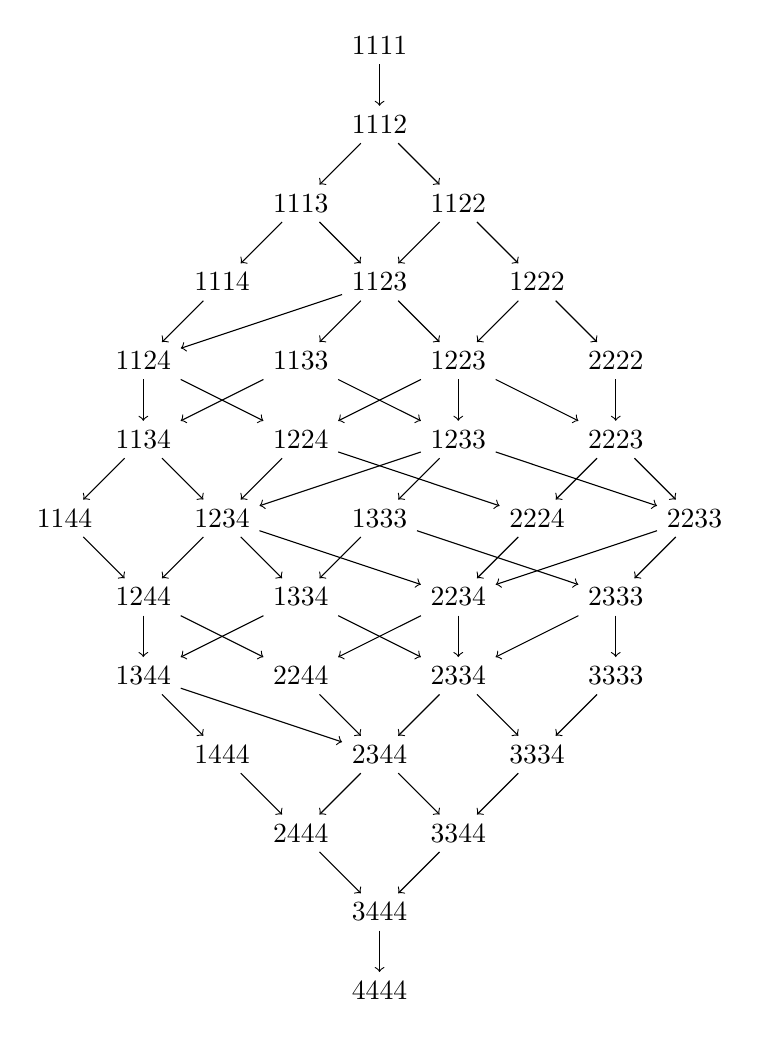
\begin{tikzpicture}
%Nodes
\node  (node1111) at (4,12) {1111};

\node  (node1112) at (4,11) {1112};

\node  (node1113) at (3,10) {1113};
\node  (node1122) at (5,10) {1122};

\node  (node1114) at (2,9) {1114};
\node  (node1123) at (4,9) {1123};
\node  (node1222) at (6,9) {1222};

\node  (node1124) at (1,8) {1124};
\node  (node1133) at (3,8) {1133};
\node  (node1223) at (5,8) {1223};
\node  (node2222) at (7,8) {2222};

\node  (node1134) at (1,7) {1134};
\node  (node1224) at (3,7) {1224};
\node  (node1233) at (5,7) {1233};
\node  (node2223) at (7,7) {2223};

\node  (node1144) at (0,6) {1144};
\node  (node1234) at (2,6) {1234};
\node  (node1333) at (4,6) {1333};
\node  (node2224) at (6,6) {2224};
\node  (node2233) at (8,6) {2233};

\node  (node1244) at (1,5) {1244};
\node  (node1334) at (3,5) {1334};
\node  (node2234) at (5,5) {2234};
\node  (node2333) at (7,5) {2333};

\node  (node1344) at (1,4) {1344};
\node  (node2244) at (3,4) {2244};
\node  (node2334) at (5,4) {2334};
\node  (node3333) at (7,4) {3333};

\node  (node1444) at (2,3) {1444};
\node  (node2344) at (4,3) {2344};
\node  (node3334) at (6,3) {3334};

\node  (node2444) at (3,2) {2444};
\node  (node3344) at (5,2) {3344};

\node  (node3444) at (4,1) {3444};

\node  (node4444) at (4,0) {4444};

%Lines
\draw[->] (node1111) edge node[thick, auto] {} (node1112);

\draw[->] (node1112) edge node[thick, auto] {} (node1113);
\draw[->] (node1112) edge node[thick, auto] {} (node1122);

\draw[->] (node1113) edge node[thick, auto] {} (node1114);
\draw[->] (node1113) edge node[thick, auto] {} (node1123);

\draw[->] (node1114) edge node[thick, auto] {} (node1124);

\draw[->] (node1122) edge node[thick, auto] {} (node1123);
\draw[->] (node1122) edge node[thick, auto] {} (node1222);

\draw[->] (node1123) edge node[thick, auto] {} (node1223);
\draw[->] (node1123) edge node[thick, auto] {} (node1124);
\draw[->] (node1123) edge node[thick, auto] {} (node1133);

\draw[->] (node1124) edge node[thick, auto] {} (node1224);
\draw[->] (node1124) edge node[thick, auto] {} (node1134);

\draw[->] (node1133) edge node[thick, auto] {} (node1233);
\draw[->] (node1133) edge node[thick, auto] {} (node1134);

\draw[->] (node1134) edge node[thick, auto] {} (node1234);
\draw[->] (node1134) edge node[thick, auto] {} (node1144);

\draw[->] (node1144) edge node[thick, auto] {} (node1244);

\draw[->] (node1244) edge node[thick, auto] {} (node1344);
\draw[->] (node1244) edge node[thick, auto] {} (node2244);

\draw[->] (node1344) edge node[thick, auto] {} (node1444);
\draw[->] (node1344) edge node[thick, auto] {} (node2344);

\draw[->] (node1444) edge node[thick, auto] {} (node2444);

\draw[->] (node2444) edge node[thick, auto] {} (node3444);

\draw[->] (node3444) edge node[thick, auto] {} (node4444);


\draw[->] (node1222) edge node[thick, auto] {} (node1223);
\draw[->] (node1222) edge node[thick, auto] {} (node2222);

\draw[->] (node1223) edge node[thick, auto] {} (node1233);
\draw[->] (node1223) edge node[thick, auto] {} (node1224);
\draw[->] (node1223) edge node[thick, auto] {} (node2223);

\draw[->] (node1224) edge node[thick, auto] {} (node1234);
\draw[->] (node1224) edge node[thick, auto] {} (node2224);

\draw[->] (node1234) edge node[thick, auto] {} (node1244);
\draw[->] (node1234) edge node[thick, auto] {} (node1334);
\draw[->] (node1234) edge node[thick, auto] {} (node2234);

\draw[->] (node1334) edge node[thick, auto] {} (node1344);
\draw[->] (node1334) edge node[thick, auto] {} (node2334);

\draw[->] (node1233) edge node[thick, auto] {} (node1333);
\draw[->] (node1233) edge node[thick, auto] {} (node1234);
\draw[->] (node1233) edge node[thick, auto] {} (node2233);

\draw[->] (node1333) edge node[thick, auto] {} (node2333);
\draw[->] (node1333) edge node[thick, auto] {} (node1334);

\draw[->] (node2222) edge node[thick, auto] {} (node2223);

\draw[->] (node2223) edge node[thick, auto] {} (node2224);
\draw[->] (node2223) edge node[thick, auto] {} (node2233);

\draw[->] (node2224) edge node[thick, auto] {} (node2234);

\draw[->] (node2233) edge node[thick, auto] {} (node2234);
\draw[->] (node2233) edge node[thick, auto] {} (node2333);

\draw[->] (node2234) edge node[thick, auto] {} (node2334);
\draw[->] (node2234) edge node[thick, auto] {} (node2244);

\draw[->] (node2334) edge node[thick, auto] {} (node2344);
\draw[->] (node2334) edge node[thick, auto] {} (node3334);

\draw[->] (node2244) edge node[thick, auto] {} (node2344);

\draw[->] (node2344) edge node[thick, auto] {} (node2444);
\draw[->] (node2344) edge node[thick, auto] {} (node3344);

\draw[->] (node3344) edge node[thick, auto] {} (node3444);

\draw[->] (node2333) edge node[thick, auto] {} (node3333);
\draw[->] (node2333) edge node[thick, auto] {} (node2334);

\draw[->] (node3333) edge node[thick, auto] {} (node3334);

\draw[->] (node3334) edge node[thick, auto] {} (node3344);
\end{tikzpicture}
\end{center}
\end{minipage}

